\chapter{Overview}\label{s:overview}
This overview contains a Utility Tree, which captures the Architecturally significant requirements (ASR). These ASRs are extracted from interviews (interviewee description in Appendix  \ref{Appendix A}) and combine with the Business Goals and Concerns (available in Appendix \ref{Appendix B} and  \ref{Appendix C}) 

\begin{table}[h!]
\centering
\begin{tabular}{||l l l||} 
 \hline
 Business Goal(s) (BG) & Concern(s) (C) & Architecturally Significant Requirement (ASR) \\ [0.5ex] 
 \hline\hline
 \makecell {BG-03} & C-03 & ASR-1 Confidentiality \\
 \hline
 \makecell {BG-01, BG-02} & C-01, C-02 & ASR-2 Re-usability\\
\hline
 \makecell {BG-05} &  C-09 & ASR-3 Maturity  \\
 \hline
\makecell {BG-04} & C-04, C-05, C-06, C-11 & ASR-4 Authenticity \\
 \hline
 \makecell {BG-01} & C-10 & ASR-5 Accountability  \\ [1ex] 
 \hline
\end{tabular}
\caption{ASRs Plotted on business goals and concerns.}
\label{ASR_BG_C}
\end{table}

Concerns C-07, C-08 and C-11 and BG-06 are not addressed in this overview because the scope of this research is not taking in account possible required changes in law and processes within non-government organizations. However, these concerns are considered possible relevant for future research and therefore included in the appendix.

 \begin{longtable}[c]{|p{4cm}|p{8cm}|p{2cm}|}
 \caption{Example of a Business Goal. Complete list available in Appendix \ref{Appendix B} Table \ref{tab:business_goals}\label{tab:Example_business_goals}}\\
 \hline
 \multicolumn{3}{| c |}{Begin of Table}\\
 \hline
 Business Goal number and name & Description & Addressed by\\
 \hline
 \endfirsthead

 \hline
 \multicolumn{3}{|c|}{Continuation of Table \ref{tab:business_goals}}\\
 \hline
 Business Goal number and name & Description & Addressed by\\
 \hline
 \endhead

 \hline
 \endfoot

 \hline
 \multicolumn{3}{| c |}{End of Table}\\
 \hline\hline
 \endlastfoot
 BG-01 Explainable solutions   &   Communicate simple how technology works to raise awareness and support. Also, provide more detailed scientific information for experts to contribute as a community. &  I-03\\
 \end{longtable}
 
 \begin{longtable}[c]{|p{4cm}|p{8cm}|p{2cm}|}
 \caption{Example of a Concern. Complete list available in Appendix \ref{Appendix C} Table \ref{tab:concerns}\label{tab:Example_concerns}}\\
 \hline
 \multicolumn{3}{| c |}{Begin of Table}\\
 \hline
 Concern number and name & Description & Addressed by\\
 \hline
 \endfirsthead

 \hline
 \multicolumn{3}{|c|}{Continuation of Table \ref{tab:business_goals}}\\
 \hline
 Concern number and name & Description & Addressed by\\
 \hline
 \endhead

 \hline
 \endfoot

 \hline
 \multicolumn{3}{| c |}{End of Table}\\
 \hline\hline
 \endlastfoot
 C-01 Knowledge of systems and what is legally allowed    &   Area of expertise within the identity domain is complex and system specialists (NL: Stelselspecialisten) and other specialists are a rare resource. History of law and systems is implicit knowledge or hard to find in documentation. When designing new systems it's needed to comprehend the domain and its internal and external influences. & I-03\\
 \end{longtable}


    
    \begin{figure}
        \graphicspath{ {./images/} }
        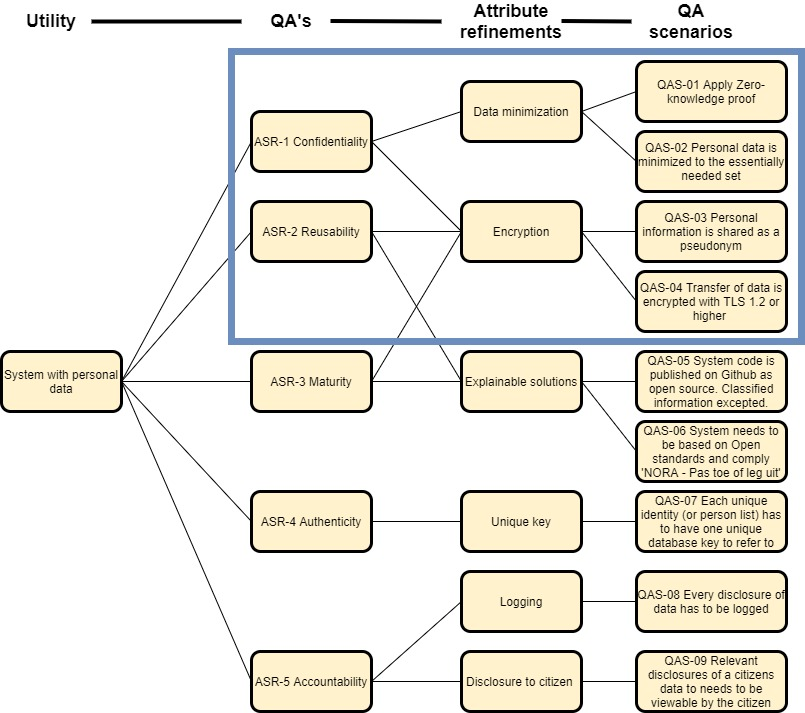
\includegraphics[width=17cm]{Decomposition of ASR and QAS-Utility Tree v3.jpg}\\
        \caption{Decomposition of Architecturally significant requirements}
        \label{fig:ASR1}
    \end{figure}